\clearpage
\section{Դինամիկ հիշողության արտահոսքի սխալների հայտնաբերում}\label{sec:bugDetection}
Ծրագրային կոդի հատկությունների հարցումների համակարգը օգտագործվել է դինամիկ հիշողության
արտահոսքեր (memory leaks)\cite{MEMORYLEAK} հայտնաբերելու համար: Այդ նպատակով, համակարգի API-ի օգտագործմամբ
իրականացվել է համապատասխան ստուգիչ (checker) (Տես Նկար \ref{fig:figure3}): Ստուգիչի աշխատանքը հիմնված է հետևյալ ալգորիթմի վրա.
\begin{enumerate}
    \item Գտնել malloc, calloc ֆունկցիաների կանչերի հրահանգները,
    \item Յուրաքանչյուր malloc, calloc կանչի համար որոշել նպատակային օպերանդը (destination),
    \item Յուրաքանչյուր նպատակային օպերանդից գտնել կախվածություն ունեցող և free կանչող հրահանգները (forward\_df\_free\_instructions),
    \item Յուրաքանչյուր ճանապարհի համար, որ սկսվում է malloc, calloc կանչից և ավարտվում է ծրագրի վերջում, ստուգել,
    արդյոք այդ ճանապարհը պարունակում է forward\_df\_free\_instructions հրահանգներից որևէ մեկը:
    \item Եթե ոչ, արձանագրել դինամիկ հիշողության արտահոսք, եթե ճանապարհն իրական է:
\end{enumerate}

\begin{figure}[h]
    \centering
    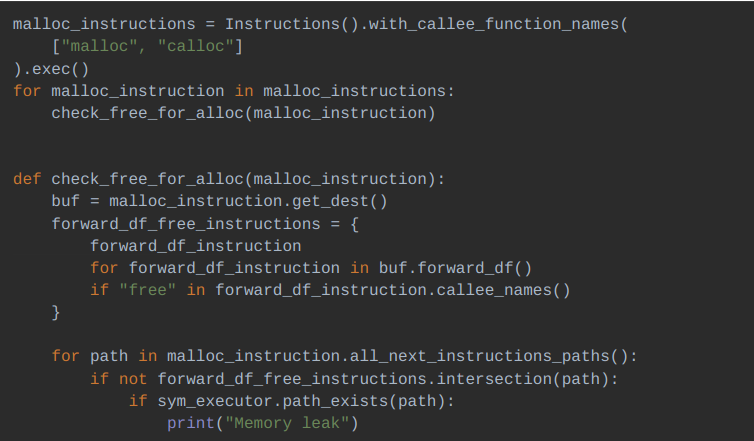
\includegraphics[width=1\textwidth]{pic3}
    \caption{Հարցումների համակարգի API-ի օգտագործմամբ գրված դինամիկ հիշողության արտահոսքի ստուգիչ}
    \label{fig:figure3}
\end{figure}

Հարցումների համակարգի օգտագործմամբ ստեղծված ստուգիչը թույլ է տալիս ավտոմատ կերպով հայտնաբերել
այնպիսի դեպքեր, երբ ծրագրի աշխատանքի ընթացքում հիշողությունը չի ազատվում ամբողջությամբ: Սա կարևոր խնդիր է ծրագրային
ապահովման որակի և արդյունավետության տեսանկյունից, քանի որ չազատված հիշողությունը կարող է հանգեցնել ծրագրի
կայունության և կատարողականության նվազեցմանը:
{
    \subsection{Թեստավորում}\label{subsec:testing}
    Մշակված գործիքը թեստավորվել և համեմատվել է աշխարհում արդեն գոյություն ունեցող այլ գործիքների հետ։ Ինչպես նաև գործիքի
    միջոցով թեստավորվել են բաց կոդով հասանելի ավելի քան 100 պրոեկտ, որոնք իրականացված են մեծամասամբ C ծրագրավորման լեզվով։

    \subsubsection{Արդյունքների համեմատումը Juliet թեստերի հավաքածույի վրա}
    MLH֊ը թեստավորվել է Juliet թեստերի հավաքածույի վրա, որը նախատեսված է ծրագրային ապահովման գործիքների թեստավորման և
    արդյունքների գնահատման համար։ Այն Software Assurance Metrics and Tool Evaluation(SAMATE)\cite{SAMATE} նախագծի մասն է
    կազմում, որը մշակվել է National Institue of Standards and Technology(NIST)֊ի կողմից։ Ջուլիետ թեստերի հավաքածուն
    ներառում է ավելի քան 120,000 թեստերի օրինակներ առանձնացված զանազան խնդիրների համար ինչպիսիք են դինամիկ հիշողության
    արտահոսքը, բուֆերի գերհագեցումը և այլն։ Այն ներառում է թեստեր C/C++, Java և Ada լեզուներով:
    Թեստավորման համար հավաքածուից առանձնացվել են միայն դինամիկ հիշողության արտահոսքի համար նախատեսված
    օրինակները (CWE401\_Memory\_Leak\cite{CWE401}): Մշակվել է թեստավորման համակարգ, որը գնահատում է ունեցած գործիքների
    արդյունավետությունը վերը նշված հավաքածուի համար։ Ստորև ներկայացված է առաջատար այլ գործիքների և
    նոր մշակված գործիքի արդյունավետության աղյուսակը (Աղյուսակ\ref{tab:juliet_test}):
    \begin{table}[h!]
    \centering
    \begin{tabularx}{\textwidth}{|*{6}{>{\centering\arraybackslash}X|}}
        \hline
        \textbf{Name} & \textbf{True Positives} & \textbf{True Negatives} & \textbf{False Positives} & \textbf{False Negatives} & \textbf{F1 score} \\
        \hline
        \textbf{CSA} & 536 & 4481 & 125 & 332 & 0.7011 \\
        \hline
        \textbf{Infer} & 262 & 4392 & 214 & 606 & 0.3899 \\
        \hline
        \textbf{SMOKE} & 496 & 4510 & 96 & 372 & 0.6795 \\
        \hline
        \textbf{PCA} & 486 & 4342 & 264 & 382 & 0.6007 \\
        \hline
        \textbf{SVF} & 452 & 4168 & 438 & 416 & 0.5142 \\
        \hline
        \rowcolor{yellow!100} \textbf{MLH} & 868 & 4606 & 0 & 0 & 1 \\
        \hline
    \end{tabularx}
    \caption{Juliet թեստերի հավաքածույի վրա համեմատման արդյունքների}
    \label{tab:juliet_test}
\end{table}
}

{
    \subsection{Արդյունքներ}\label{subsec:results}
    Ստորև ներկայացված է առաջատար այլ գործիքների և
    նոր մշակված գործիքի արդյունավետության աղյուսակը (Աղյուսակ\ref{tab:juliet_test}):
    \begin{table}[h!]
    \centering
    \begin{tabularx}{\textwidth}{|*{6}{>{\centering\arraybackslash}X|}}
        \hline
        \textbf{Name} & \textbf{True Positives} & \textbf{True Negatives} & \textbf{False Positives} & \textbf{False Negatives} & \textbf{F1 score} \\
        \hline
        \textbf{CSA} & 536 & 4481 & 125 & 332 & 0.7011 \\
        \hline
        \textbf{Infer} & 262 & 4392 & 214 & 606 & 0.3899 \\
        \hline
        \textbf{SMOKE} & 496 & 4510 & 96 & 372 & 0.6795 \\
        \hline
        \textbf{PCA} & 486 & 4342 & 264 & 382 & 0.6007 \\
        \hline
        \textbf{SVF} & 452 & 4168 & 438 & 416 & 0.5142 \\
        \hline
        \rowcolor{yellow!100} \textbf{MLH} & 868 & 4606 & 0 & 0 & 1 \\
        \hline
    \end{tabularx}
    \caption{Juliet թեստերի հավաքածույի վրա համեմատման արդյունքների}
    \label{tab:juliet_test}
\end{table}

    \subsubsection{Դինամիկ հիշողության արտահոսքի հայտնաբերումը առաջատար բաց կոդով գործիքներում}
    Մի շարք հատուկ առանձնացված բաց կոդով գործիքներ դասակարգված են ըստ իրենց ակտիվության և կարևորության։ Այդ գործիքներից
    ավելի քան հարյուրը թեստավորվել են նոր մշակված գործիքի միջոցով՝ դինամիկ հիշողության արտահոսքի խնդիրները հայտնաբերելու
    նպատակով։ Ստացված արդյունքները հավելյալ ստուգվել են աշխատակիցների կողմից։ Ստացված ճիշտ արդյունքները հրապարակվել և
    հաստատվել են, սխալ ստացված արդյունքների համար կատարվել է վերլուծություն և մշակվել հետագա պլան գործիքում առկա
    թերությունները վերացնելու նպատակով։ Նկար \ref{fig:figure4}-ում ներկայացված է ֆունկցիայի օրինակ
    coturn\cite{COTURN}-ից, որում հարցումների համակարգի API-ի օգտագործմամբ գրված
    սստուգիչի կողմից հայտնաբերվել է դինամիկ հիշողության արտահոսքի դեպք։

    \begin{figure}[h]
        \centering
        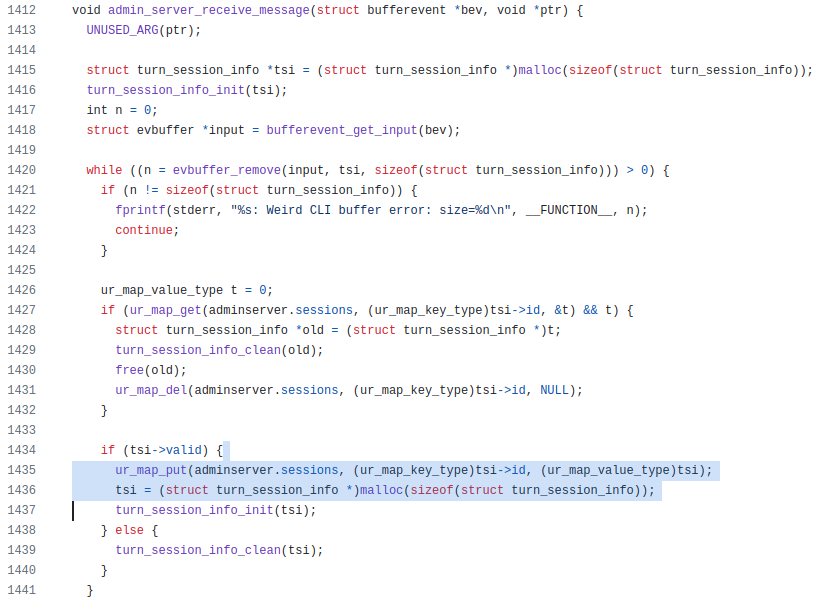
\includegraphics[width=1\textwidth]{pic4}
        \caption{Դինամիկ հիշողության արտահոսքի իրական օրինակ}
        \label{fig:figure4}
    \end{figure}
}